
\documentclass[11pt]{article}

\usepackage[a4paper,pdftex]{geometry}	
\usepackage[slovak]{babel}
\usepackage{xcolor} 
\usepackage{fix-cm} 


\usepackage{graphicx}

\usepackage[utf8]{inputenc}

\usepackage{url}
\usepackage{hyperref}

\usepackage{listings}

\usepackage{enumitem}

\setlength{\oddsidemargin}{0mm} 
\setlength{\evensidemargin}{0mm} 

\newcommand{\HRule}[1]{\hfill \rule{0.2\linewidth}{#1}} 
\newcommand{\lsti}{\lstinline}
\definecolor{grey}{rgb}{0.9,0.9,0.9} 	

\usepackage{fancyhdr}

\pagestyle{fancy}
\fancyhf{}
\rhead{}
\lhead{ \leftmark }
\rfoot{Strana \thepage}

\usepackage{amsmath}


\usepackage{listings,color}

\definecolor{verbgray}{gray}{0.9}

\lstnewenvironment{code}{%
  \lstset{backgroundcolor=\color{verbgray},
  frame=single,
  framerule=0pt,
  basicstyle=\ttfamily,
  columns=fullflexible}}{}

\definecolor{shadecolor}{rgb}{.9, .9, .9}

\newif\ifknowhow
\newcommand{\ommited}{ VYNECHANÉ }

\begin{document}

%----
% COMMENT IF KNOW HOW SHOULD BE OMMITED
%----
\knowhowtrue
  





\thispagestyle{empty} 

%----------------------------------------------------------------------------------------
%	TITLE SECTION
%----------------------------------------------------------------------------------------

\colorbox{grey}{
	\parbox[t]{1.0\linewidth}{
		\centering \fontsize{50pt}{80pt}\selectfont
		\vspace*{0.7cm} 
		
		\hfill Architektúra \\
		\hfill Náklady \\
		\hfill Soundslash  \\
		%\hfill \par
		
		\vspace*{0.7cm} 
	}
}

%----------------------------------------------------------------------------------------

\vfill 

{\centering \large
\ifknowhow 
\else \hfill V tomto dokumente boli vynechané časti.\\ \fi 
\hfill \today \\
\hfill Michal Bystrický \\
\hfill \href{mailto:bystricky@soundslash.com}{bystricky@soundslash.com} \\

\HRule{1pt}} 

%----------------------------------------------------------------------------------------

\clearpage 


\tableofcontents


\clearpage

\section{Úvod}

Tento dokument opisuje architektúru služby Soundslash a architektúru nasadenia. Jeho cieľom je vypočítať náklady na prevádzku služieb Soundslash pri danej architektúre. Opiera sa o dostupné metriky a zdroje vďaka ktorým počíta veľmi približnú kalkulácia nákladov pre jednotlivé služby.


\section{Aktuálny Stav Architektúry}

Táto sekcia opisuje aktuálny stav architektúry. Sekcia \ref{hlp1} opisuje hlavný prípad použitia na úrovni summary (strategic) cieľov a konsekventne Sekcia \ref{hlp3} architektúru za ním. Sekcia \ref{hlp2} sa venuje typom služieb z pohľadu architektúry. Sekcia \ref{os} dodáva k hlavnému prípadu použitia ďalšie dôležité architektonické rozhodnutia.


\subsection{Hlavný Prípad Použitia \label{hlp1}}

Hlavný prípad použitia predstavuje vytvorenie internetového rádia a jeho manažment. Teda mohli by sme povedať, že na úrovní strategických cieľov sa tento prípad použitia bude volať ``Správa rádia''. Voľne ho môžeme opísať nasledovnými krokmi:

\begin{enumerate}[noitemsep]
\item Organizácia vyberie ``Vytvorenie rádia''
\item Systém vytvorí rádio
\item Systém spustí rádio
\item System umožní organizácii rádio spravovať
\item Systém umožní rádio počúvať
\item Organizácia nahrá média
\item Organizácia vytvára program
\item Organizácia robí LIVE vstupy
\item Poslucháč počúva rádio
\end{enumerate}

\subsection{Typy Služieb \label{hlp2}}

Z pohľadu architektúry existujú 2 typy služieb:

\begin{itemize}[noitemsep]
\item re-enkódované,
\item enkódované.
\end{itemize}

Ak ide o re-enkódovaný stream, média sa dekódujú, mixujú a enkódujú za behu. Takto napríklad môžeme primixovať LIVE stopu priamo z mikrofónu, alebo realizovať fade efekt na audio stopu. Pri enkódovaných nie je potreba tohto processingu, pretože už sú média spracované a posielajú sa priamo poslucháčom. Avšak, pri enkódovanom type nie je možné mixovať alebo inak upravovať stream.

\subsection{Architektúra a Hlavný UC \label{hlp3}}

Teraz si prejdeme architektúru za týmto prípadom použitia. Služba Soundslash je škálovateľná. Na Obrázku \ref{ss01} môžeme vidieť architektúru a rozloženie záťaže. Treba si uvedomiť, že \ifknowhow každý komunikuje s každým na lokálnej sieti (nie nevyhnutne), okrem Web a Auth serverov. \else\ommited{}\fi Ako identifikátor aplikácia vie svoju lokálnu IP a verejnú IP.

DMZ nie je prístupná z Internetu, teda používatelia sa pripájajú na load balancer a Icecast streaming servery. Ďalej, load balancer rozloží záťaž na web servery, \ifknowhow kde sa realizuje aj encoding audio súborov. Ak je encoding dokončený pridá sa tento audio súbor do databázy MongoDB\else\ommited{}\fi. Média spolu s programom sa ukladajú do databázy.

\begin{figure}[htp]
\centering

\ifknowhow
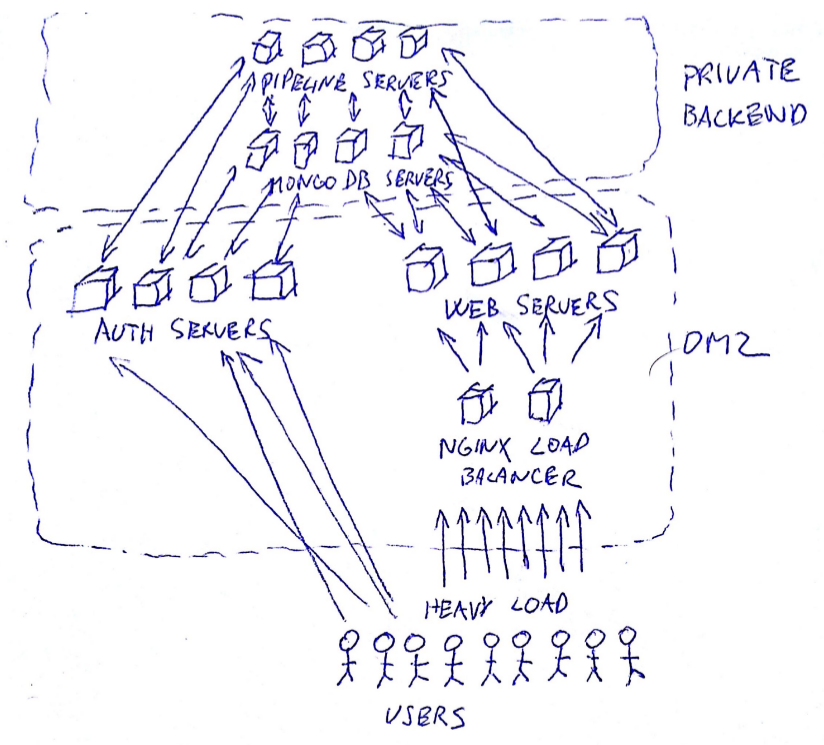
\includegraphics[scale=0.30]{01.png}
\else\ommited{}\fi

\caption{Architektúra služby Soundslash}
\label{ss01}
\end{figure}


Asynchrónne z tejto databázy \ifknowhow podľa programu, sú média vyberané, (dekódované, mixované, enkódované---v závislosti od typu služby) a posielané do Auth serverov\else\ommited{}\fi. Na Auth serveroch beží streaming server Icecast, ktorý aktualizuje tabuľku streamov k serverom v databáze. Teda, ak už je poslucháčov mnoho Auth aktualizuje túto tabuľku. Následne pri pripojení ďalšieho poslucháča podľa tabuľky buď (1) pošle Web server požiadavku na Pipeline o pripojení ďalšieho Auth servera (2) alebo v prípade, že Auth server nie je plný, tak ho pripojí na tento server.  

Teda, Pipeline realizuje samotné škálovanie (pripájanie) Auth serverov, pretože on realizuje samotný stream. Aby používateľ mohol ovládať stream, Pipeline má 2 interfejsi, ako môžeme vidieť na Obrázku \ref{ss02}. Prvý HTTP API prijíma správy, ktoré ovládajú stream, druhý Websockets slúži na posielanie LIVE dát z mikrofónu.

\begin{figure}[htp]
\centering
\ifknowhow
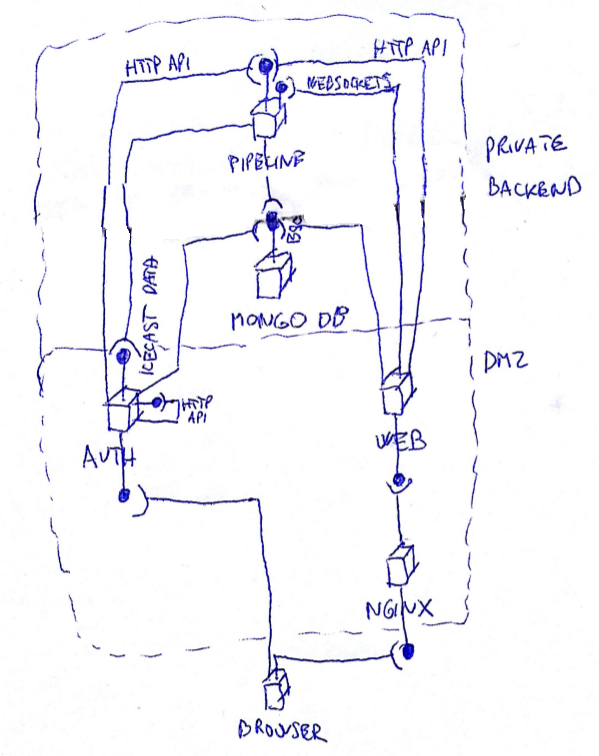
\includegraphics[scale=0.35]{02.png}
\else\ommited{}\fi
\caption{Interfejsi služby Soundslash}
\label{ss02}
\end{figure}

Na serveroch Auth \ifknowhow beží Icecast streaming server, ktorý počúva a prijíma stream, ktorý ďalej distribuuje poslucháčom. Server Icecast cez HTTP API komunikuje s Auth serverom o streamoch, teda, \else\ommited{}\fi aktualizuje mu nasledovné:

\begin{itemize}[noitemsep]
\item pridanie nového streamu,
\item odpojenie streamu,
\item pripojenie poslucháča,
\item odpojenie poslucháča.
\end{itemize}

Auth server potom na základe týchto informácii aktualizuje tabuľku o dostuponosti Icecast streaming serverov, ktorej príklad môžeme vidieť v prílohe \ref{sec:tab}. Atribút level je od stupňa 0 do 10, kde 10 predstavuje úplne plný server a 0 práve vytvorený. Tento atribút je aktualizovaný pri Pipeline podľa CPU a pri Auth podľa poslucháčov.

\subsection{Opis Serverov  \label{os}}

\paragraph{Pipeline server.} Hlavná úloha je práca so streamom, \ifknowhow teda dekódovanie, mixovanie, enkódovania a pripájanie nových Icecast streaming serverov. Tento server si sám aktualizuje tabuľku o vyťaženosti \else\ommited{}\fi (atribút \texttt{level}). Ak je moc vyťažený ďalšie streamy nespúšťa. Web server potom hľadá iný menej-vyťažený, ak je nenájdený, používateľovi je oznámený problém o nedostatku serverov. 

Metódy, ktoré je možné spúšťať na Pipeline HTTP API:

\ifknowhow
\begin{code}
(r"/live.json", LiveHandler),
(r"/updates.json", UpdatesHandler),
(r"/start-streaming.json", StartStreamHandler),
(r"/restart.json", RestartStreamHandler),
(r"/scale.json", ScaleHandler),
(r"/is-alive.json", IsAliveHandler),
(r"/playlist-update.json", PlaylistUpdateHandler),
(r"/run-command.json", RunCommandHandler)
\end{code}
\else\ommited{}\fi

Posledná metóda umožňuje spúšťať príkazy z webového rozhrania a to sú nasledovné:

\begin{itemize}[noitemsep]
\item use, dump\_dot\_file, start, stop, next, scale, rescale, playlist
\end{itemize}

\paragraph{Auth server.} Jeho hlavná úloha je \ifknowhow autentifikácia poslucháčov. Icecast streaming server sa pýta priamo tohto servera cez HTTP API, či poslucháčovi pustiť stream alebo nie. Aktualizuje tabuľku o Icecast streaming serveroch a ak Pipeline prestane posielať stream, opýta sa ho, či je dostupný, ak nie je, \else\ommited{}\fi tak ho označí za nedostupný. 

Metódy, ktoré je možné spúšťať na Auth HTTP API:

\ifknowhow
\begin{code}
(r"/mount_add", MountAddHandler),
(r"/mount_remove", MountRemoveHandler),
(r"/listener_add", ListenerAddHandler),
(r"/listener_remove", ListenerRemoveHandler),
\end{code}
\else\ommited{}\fi

\paragraph{Web server.} Ak Pipeline nie je dostupný označí ho za nedostupný. Získava \ifknowhow dáta o dosupnosti z tabuľky o dostupnosti z databázy (server MongoDB). Odosiela správu na spustenie nového streamu, alebo na spustenie nového Icecast streaming servera, \else\ommited{}\fi ak je to potrebné. 


\begin{figure}[htp]
\centering
\ifknowhow
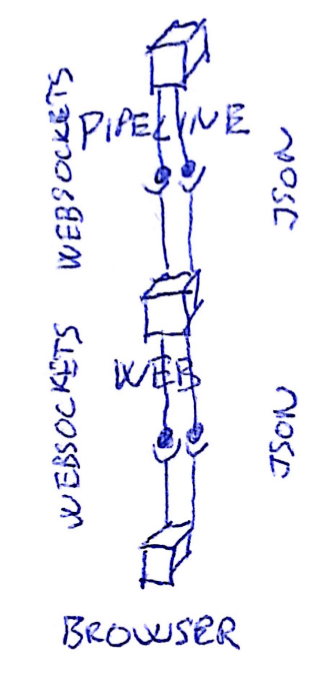
\includegraphics[scale=0.23]{04.png}
\else\ommited{}\fi
\caption{Detail Web server}
\label{ss03}
\end{figure}

Na Obrázku \ref{ss03} môžeme vidieť detail, ako Web server komunikuje s prehliadačom. Web server poskytuje iba datovú vrstvu nad databázou (JSON), teda celý obsah je generovaný na strane klienta. \ifknowhow Ide o tučného klieta, kde URL routing, generovanie frontendu a logika aplikácie je presunutá ku klientovi. Server iba odpovedá na požiadavky, ktoré nevyhnutne potrebujú databázu alebo pripojenie k Pipeline. Websockets interfejs je požitý \else\ommited{}\fi na aktualizáciu piesní pomocou vzoru Observer a tiež na odosielanie dát z mikrofónu. 

\section{Testovacie Servery}

Táto sekcia opisuje servery na ktorých budú robené testy a tiež diskutuje minimálne konfigurácie pre jednotlivé typy serverov. Sekcia \ref{fs} predstavuje fyzický server, na ktorom bude umiestnený virtuálny server (VPS) opísaný v Sekcii \ref{vps}.

\subsection{Fyzický Server \label{fs}}

Fyzický server má 2x CPU po 8 vláknach, čo je spolu 16 jadier. Na stroji je 16x VPS virtualizované na technológii KVM. Tabuľka \ref{fs02} prehľadne zobrazuje konfiguráciu fyzického servera. Na tomto fyzickom serveri je umiestnená 1x VPS opísaná Sekcii \ref{vps}.

\begin{table}[htp]
\centering
\begin{tabular}{|l|l|}
\hline
	CPU & 2x 2266.746 MHz\\
\hline
	Cores & 2x8=16\\
\hline
\end{tabular}
\caption{Fyzický server}
\label{fs01}
\end{table}


\subsection{VPS \label{vps}}

Tabuľka \ref{fs02} prehľadne zobrazuje minimálnu konfiguráciu spustenia služby na 1 VPS. Pozri Sekciu \ref{min} pre viac informácii.

\begin{table}[htp]
\centering
\begin{tabular}{|l|l|}
\hline
	Cores & 2\\
\hline
	RAM & 512 MB\\
\hline
	HDD & 40 GB\\
\hline
\end{tabular}
\caption{VPS}
\label{fs02}
\end{table}


\section{Minimálne Konfigurácie \label{min}}

Táto sekcia sa venuje minimálnym konfiguráciam. Sekcia \ref{oh} diskutuje o všeobecných ohraničeniach. Sekcia \ref{oh2} následne opisuje optimálne konfigurácie pre jednotlivé servery.



\subsection{Všeobecné Ohraničenia \label{oh}}

\paragraph{CPU.} Minimálna konfigurácia CPU je minimálne 2 jadrá (pokiaľ máme celú aplikáciu na na 1 VPS), pretože server Pipeline si aktualizuje svoje vyťaženie na základe CPU a teda počas processingu médii by sa mohol označiť ako plne využitý a už ďalej nespúšťať nové rádiá. Teda hneď po vytvorení rádia (po processingu prvej audio stopy) by nebolo spustené. 

\paragraph{HDD.} Operačný systém spolu so softvérom, aplikáciou a knižnicami je veľký do 5 GB, ako je vidno v prílohe \ref{sec:knf}. Teda minimálna veľkosť na diskový priestor je 5 GB (bez akejkoľvek databázy).

\paragraph{RAM.} Podľa prílohy \ref{sec:knf} minimum pre spustenie aplikácie je 256 MB RAM.

\paragraph{Traffic.} Sieťová prevádzka závisí od počtu poslucháčov. Pri 8 hodinovom počúvaní denne, 1 rádio, 10 poslucháčov, 128 kbps za mesiac je to 2.3 GB. Tabuľka \ref{tra} prehľadne zobrazuje ďalšie variácie.

\begin{table}[htp]
\centering
\begin{tabular}{|p{2cm}|p{2cm}|p{2.5cm}|p{2cm}|p{2cm}|}
\hline
	Počet rádií & Poslucháčov & Čas počúvania [h/d] & Bitrate [kbps] & Traffic [GB/mes]\\
\hline
	1 & 1 & 8 & 128 & 0.225\\
\hline
	1 & 300 & 8 & 128 & 66\\
\hline
	10 & 1 & 8 & 128 & 2.3\\
\hline
	10 & 100 & 8 & 128 & 220\\
\hline
	100 & 100 & 8 & 128 & 2 200\\
\hline
	100 & 300 & 8 & 128 & 6 600\\
\hline
	100 & 300 & 8 & 256 & 132 000\\
\hline
\end{tabular}

\caption{Traffic}
\label{tra}
\end{table}

\subsection{Optimálne konfigurácie \label{oh2}}

Táto sekcia rozoberá optimálne konfigurácie v závislosti od typov serverov. 

\paragraph{Pipeline.} Pipeline je server, kde beží mnoho \ifknowhow GStreamer\else\ommited{} \fi  vlákien, preto vhodným nastavením by bola konfigurácia s viacerími jadrami. Pre VPS zostavu sme vykonali test, ktorého výsledky možno vidieť v Tabuľke \ref{red1}. Treba upozorniť, že testovacia zostava je 2 jadrová, teda ak jedno jadro je vyťažené na 100\% a druhé na 0\%, výsledne bude 50\% záťaž. Opäť, ak budeme mať silnejšie alebo slabšie fyzické CPU, záťaž sa môže líšiť.

\begin{table}[htp]
\centering
\begin{tabular}{|p{2cm}|p{2cm}|p{2cm}|p{2cm}|p{2cm}|p{2cm}|}
\hline
	Počet reencoding & Počet encoding & Dĺžka testu [min] & CPU AVG [\%] & CPU MAX [\%] & RAM [\%]\\
\hline
	1 & 0 & 2 & 7.308 & 12 & 59.2\\
\hline
	1 & 1 & 2 & 9.233 & 14 & 64.5\\
\hline
	2 & 1 & 2 & 15.3 & 23 & 66.8 \\
\hline
	2 & 2 & 2 & 16.6 & 24 & 69.5 \\
\hline
	3 & 2 & 2 & 22.7 & 30 & 74 \\
\hline
	4 & 2 & 2 & 28.9 & 41 & 77.4 \\
\hline
	5 & 2 & 2 & 33 & 47 & 81 \\
\hline
\hline
	0 & 1 & 2 & 1.6 & 4 & 65.1 \\
\hline
	0 & 2 & 2 & 2.9 & 8 & 66.1\\
\hline
	0 & 3 & 2 & 1.76 & 4 & 67.6 \\
\hline
	0 & 4 & 2 & 4 & 8 & 69.2 \\
\hline
	0 & 5 & 2 & 2.05 & 6 & 71 \\
\hline
	0 & 6 & 2 & 2.03 & 5 & 72.3 \\
\hline
\end{tabular}

\caption{Pipeline server test}
\label{red1}
\end{table}

Mohli by sme predpokladať, že 8\% CPU je vyžadovaného na 1 reencoding stream pri danej zostave. RAM stúpala o cca 5\%, čo je cca 26 MB. Základ pamäte RAM je 59\%, čo predstavuje 300 MB. Nasledovná tabuľka prehľadne opisuje požiadavky na 1 re-encoding stream.

\begin{center}
\begin{tabular}{|l|l|}
\hline
	CPU & 8\%\\
\hline
	RAM & 26 MB\\
\hline
\end{tabular}
\end{center}

Daným pomerom získame optimálnu konfiguráciu. Na dané CPU sa zmestí cca 10-12 re-encoding streamov, pričom pre 12 streamov potrebujeme 300+(12*26) = 612 MB RAM. Preto optimálna zostava pre Pipeline server je uvedená v Tabuľke \ref{konf1}.

\begin{table}[htp]
\centering
\begin{tabular}{|l|l|}
\hline
	Cores & 2\\
\hline
	RAM & 756 MB\\
\hline
	HDD & 5 GB\\
\hline
	Počet re-encoding & 10-12\\
\hline
	Percentuálne 1 re-encoding & 0.1 \%\\
\hline
\end{tabular}
\caption{Optimálna konfigurácia Pipeline servera (re-encoding 64 kbps)}
\label{konf1}
\end{table}

Ďalej by sme mohli predpokladať, že 1.5\% CPU je vyžadovaného na 1 encoded stream pri danej zostave. Pamäť RAM sa zvyšuje o cca 2\%, čo je 11 MB. Základ bol 65\%, čo je 333 MB RAM. Nasledovná tabuľka opisuje požiadavky na 1 encoded stream.


\begin{center}
\begin{tabular}{|l|l|}
\hline
	CPU & 1.5\%\\
\hline
	RAM & 11 MB\\
\hline
\end{tabular}
\end{center}

Podľa tohto pomeru, pre encoded stream sa zmestí na daný VPS server 60-65 streamov, pričom pamäť RAM v závislosti od tohto by bola 333+(65*11) = 1024 MB RAM. Mohli by sme špekulovať, že 756 MB RAM je tiež akceptovateľné, nakoľko merania pamäte RAM obsahujú aj cache RAM. Preto optimálna zostava pre Pipeline server je uvedená v Tabuľke \ref{konf2}.

\begin{table}[htp]
\centering
\begin{tabular}{|l|l|}
\hline
	Cores & 2\\
\hline
	RAM & 1024 MB (756 MB)\\
\hline
	HDD & 5 GB\\
\hline
	Počet encoded & 60-65\\
\hline
	Percentuálne 1 encoded & 0.017 \%\\
\hline
\end{tabular}
\caption{Optimálna konfigurácia Pipeline servera (encoded 64 kbps)}
\label{konf2}
\end{table}






\paragraph{Auth.} Server Auth úzko spolupracuje s Icecast streaming serverom pomocou HTTP API, ktoré Auth poskytuje všetko na 1 node. Preto musíme rátať s určitým prídavným zaťažením (overhead-om) okrem Icecast zaťaženia, ktoré je zanedbateľné, pretože ide o requesty do databázy. Odrazíme sa od testov \footnote{http://icecast.org/loadtest/1/} a \footnote{http://icecast.org/loadtest/2/}, limitujúce faktory sú nasledovné:

\begin{itemize}[noitemsep]
\item Sources. Každý source pridáva cca 1 MB RAM (672 KB).
\item Traffic vs Listeners. Poslucháči nemajú vplyv na hardwarovú zostavu, práve traffic je limitujúci faktor. V teste, pri 14 000 poslucháčov narazili práve na limit trafficu.  
\end{itemize}

Pipeline posiela dáta do sources, ktoré sú po 8 poslucháčov (čím menej poslucháčov v sources, tým presnejšie využitie sources). Ak sa na stream pripojí viac ako 8 poslucháčov Pipeline začne posielať audio dáta do ďalšieho source. Teda, ak rátame s nasledovným limitom, pre 512 MB RAM, kde základ je 300 MB sa nám zmestí cca 200 sources po 8 poslucháčov.

Ak by ste mali 10 Mbit/s sieť (= 1 250 kB/s = 1.25 MB) upload. Do tohto rozsahu sa nám zmestí 78 streamov pri 128 kbit/s. Tabuľka \ref{kon} zobrazuje ďalšie variácie.

\begin{table}[htp]
\centering
\begin{tabular}{|ll|l|l|l|l|}
\hline
	           & & 10 Mbit/s & 100 Mbit/s & 1 Gbit/s & 10 Gbit/s \\
%	           & & (1 250 kB/s) & (12 500 kB/s) & (125 000 kB/s) & (1 250 000 kB/s) \\
\hline
	64 kb/s  & (8 kB) & 156   & 1 562     & 15 625   & 156 250\\
	
	           &          & 19/9/4 & 195/97/48 & 1 953/976/488  & 19 531/9 765/4 882\\
\hline
	128 kb/s & (16 kB) & 78        & 781        & 7 812    & 78 125 \\
	           &          & 9/4/2 & 97/48/24 & 976/488/244  & 9 765/4 882/2 441\\
\hline
	256 kb/s & (32 kB) & 39       & 390        & 3 906    & 39 062\\
	           &       & 4/2/1 & 48/24/12 & 488/244/122  & 4 882/2 441/1 220\\
\hline
\end{tabular}
\caption{Počet maximum konkurentných streamov pri rôznych rozsahoch siete. V druhom riadku môžeme vidieť koľko sources po 8/16/32 poslucháčov, čo sú aj požiadavky na pamäť RAM v MB.}
\label{kon}
\end{table}

Ako je možné vidieť z tabuľky pre VPS, ktorá má 512 MB RAM a 128 kbit/s streamoch, by sme vedeli pri základe 300 MB RAM vytvoriť 200 sources po 8 poslucháčov, ktoré by obslúžili 1 600 poslucháčov, museli by sme však mať cca 3x 100 Mbit/s upload. Teda, ako je vidieť z tabuľky, naozaj, limitujúci faktor je primárne traffic.

Tabuľka \ref{kon2} poskytuje iný pohľad podľa poslucháčov. Základ 200 MB by sme zarátali pri novom stroji, teda každých cca 750 (256 MB RAM), alebo 2 500 (512 MB RAM), alebo 5 000 poslucháčov (1 024 MB RAM). Teda pri prvej najneoptimálnejšej alternatíve by na 1 poslucháča vychádzalo zo zostavi 0.002 percenta, pri druhej 0.0004 \% a pri tretej 0.0002 \%. V Tabuľke \ref{konf2} možno vidieť optimálnu konfiguráciu Auth servera.

\begin{table}[htp]
\centering
\begin{tabular}{|l||l|l|}
\hline
	Poslucháči & Traffic [Mbit/s] & Počet sources/RAM [MB]\\
\hline
	1      & 0.128 & 1\\
\hline
	8      & 1.024 & 1\\
\hline
	50     & 6.4 & 7\\
\hline
	100    & 12.8 & 13\\
\hline
	300    & 38.4 & 38\\
\hline
	750    & 96 & 93\\
\hline
	1 000  & 128 & 125\\
\hline
	2 500  & 320 & 312 \\
\hline
	5 000  & 640 & 625\\
\hline
	10 000 & 1 280 & 1 250\\
\hline
\end{tabular}
\caption{Požiadavky na traffic a RAM podľa poslucháčov pre 128 kbit/s stream. }
\label{kon2}
\end{table}







\begin{table}[htp]
\centering
\begin{tabular}{|l|l|l|l|}
\hline
	Cores & 1 & 1 & 1\\
\hline
	RAM & 256 MB & 512 MB & 1 024 MB\\
\hline
	HDD & 5 GB & 5 GB & 5 GB\\
\hline
	Traffic (64 kbps) & 48 Mbit/s & 160 Mbit/s & 320 Mbit/s\\
\hline
	Traffic (128 kbps) & 96 Mbit/s & 320 Mbit/s & 640 Mbit/s\\
\hline
	Traffic (256 kbps) & 192 Mbit/s & 640 Mbit/s & 1 280 Mbit/s\\
\hline
	Počet poslucháčov & 750 & 2 500 & 5 000 \\
\hline
	Percentuálne 1 poslucháč & 0.002 \% & 0.0004 \% & 0.0002 \%\\
\hline
\end{tabular}
\caption{Optimálna konfigurácia Auth servera}
\label{konf2}
\end{table}





\paragraph{Web.} Ako sme už pokázali aplikácia je hrubý klient, preto po vybraní dát z databázy nie je takmer vôbec s nimi manipulované ďalej. Avšak, signifikantná záťaž je na processing médií, ktorej sa budeme venovať. 

Pre jedno vlákno a pre danú VPS zostavu sme testovali nahrávanie a processing médií v Tabuľke \ref{testproc}. Mohli by sme predpokladať, že na danej zostave 5 minútové audio sa processuje do 30 sekúnd. Preto ak jeden album, ktorý obsahuje 10 audio stôp, je nahrávaný, dĺžka trvania nahrávania je cca 5 minút.

\begin{table}[htp]
\centering
\begin{tabular}{|l|l|l|l|}
\hline
	Názov                 & Veľkosť [M] & Dĺžka [m:s] & Čas [sec]\\
\hline
	Skin \& Bones.mp3     & 3.0 & 4:17 & 20\\
\hline
	Home.mp3              & 5.4 & 5:50 & 28\\
\hline
	Always In My Head.mp3 & 8.3 & 3:36 & 21\\
\hline
	Politik.mp3           & 16  & 6:53 & 42\\
\hline
\end{tabular}
\caption{Testovanie processingu médií (aj s nahrávaním 10 Mbit/s upload do 1-4 sec a spustením streamu do 1 sec)}
\label{testproc}
\end{table}


Teda daná VPS zostava pri 1 vlákne dokáže spracovať za 1 deň cca 2 800 médií (kde každá audio stopa je dlhá približne 5 minút). Ak počítame, že jedno rádio nahrá 1 album za 2 dni (čo je cca 10 audio stôp), tak za mesiac nahrá 150 médií, čo je 5\%. Preto optimálna zostava je uvedená v Tabuľke \ref{konf3}.



\begin{table}[htp]
\centering
\begin{tabular}{|l|l|l|l|}
\hline
	Cores & 1 \\
\hline
	RAM & 512 MB \\
\hline
	HDD & 5 GB \\
\hline
	Percentuálne 1 rádio/mesiac & 5\% \\
\hline
\end{tabular}
\caption{Optimálna konfigurácia Web servera}
\label{konf3}
\end{table}

\paragraph{MongoDB.} K databáze pristupujú Web, Pipeline a Auth servery. Indexované kľúče sú v pamäti RAM, ktorá teda koreluje s počtom dát, ktoré majú index. Dáta sú na disku. Preto, limitujúce faktory sú:

\begin{itemize}[noitemsep]
\item Počet requestov.
\item Veľkosť disku. Pre jedno rádio odhad podľa oddychovka.eu 30 GB.
\item Veľkosť RAM podľa veľkosti indexov. 
\end{itemize}   

Pri používaní systému sme namerali 300 queries za cca 5 minút, čo je 1 query/s. Najdlhšia query bola 75 ms pri malých dátach (10 malých rádií). Tendencia je udržať dĺžku query do 100 ms pomocou indexov. Preto, optimálna konfigurácia MongoDB servera je v Tabuľke \ref{konf4}. Testy sú v prílohe \ref{poyu}.


\begin{table}[htp]
\centering
\begin{tabular}{|l|l|l|l|}
\hline
	Cores & 1 \\
\hline
	RAM & 512 MB \\
\hline
	HDD & 5+(30*10) = 305 GB \\
\hline
	Percentuálne 1 rádio/mesiac & 0.1\% \\
\hline
\end{tabular}
\caption{Optimálna konfigurácia MongoDB servera}
\label{konf4}
\end{table}

\section{Cenové Ponuky}

Táto sekcia opisuje cenové ponuky pre servery.

\subsection{VPSTech}

V Tabuľke \ref{sumkonf} je cenová ponuka VPSTech.


\begin{table}[htp]
\centering
\begin{tabular}{|l|p{4cm}|l|}
\hline
	Názov & Konfigurácia & Cena \\
\hline
	Server Pipeline & 
	Cores: 2 \newline
	RAM: 756 MB \newline
	HDD: 5GB
	& 12 E/mes
	\\
\hline
	Server Auth &
	Cores: 1 \newline
	RAM: 256 MB \newline
	HDD: 5GB \newline
	Traffic: 48 Mbit/s
	& 6 E/mes
	\\
\hline
	Server Web &
	Cores: 1 \newline
	RAM: 512 MB \newline
	HDD: 5GB
	& 8 E/mes
	\\
\hline
	Server MongoDB &
	Cores: 1 \newline
	RAM: 512 MB \newline
	HDD: 305 GB
	& 44 E/mes
	\\
\hline
	Server MongoDB variácia 1 &
	Cores: 1 \newline
	RAM: 512 MB \newline
	HDD: 35 GB
	& 17 E/mes
	\\
	
\hline
	Core upgrade  & 1 to 2 & 1.5 E/mes \\
\hline
	Core upgrade  & 2 to 4 & 2 E/mes \\
\hline
	RAM upgrade & +256 MB RAM & 2 E/mes \\
\hline
	RAM upgrade & +512 MB RAM & 4 E/mes \\
\hline
	HDD upgrade & +30 GB HDD & 9 E/mes \\
\hline
\end{tabular}

\caption{VPSTech cenová ponuka}
\label{sumkonf}
\end{table}



\subsection{WebSupport}

V Tabuľke \ref{sumkonf2} je cenová ponuka WebSupport. WebSupport neumožňuje rezervovať traffic a navyše maximálne HDD je 200 GB.  

\begin{table}[htp]
\centering
\begin{tabular}{|l|p{4cm}|l|}
\hline
	Názov & Konfigurácia & Cena \\
\hline
	Server Pipeline & 
	Cores: 2 \newline
	RAM: 756 MB \newline
	HDD: 5GB
	& 13.28 E/mes
	\\
\hline
	Server Auth &
	Cores: 1 \newline
	RAM: 256 MB \newline
	HDD: 5GB \newline
	Traffic: 48 Mbit/s (!)
	& 6.61 E/mes
	\\
\hline
	Server Web &
	Cores: 1 \newline
	RAM: 512 MB \newline
	HDD: 5GB
	& 9.46 E/mes
	\\
\hline
	Server MongoDB &
	Cores: 1 \newline
	RAM: 512 MB \newline
	HDD: 305 GB (200)
	& 80 E/mes
	\\
\hline
	Core upgrade  & 1 to 2 & 1.36 E/mes \\
\hline
	Core upgrade  & 2 to 4 & 2.21 E/mes \\
\hline
	RAM upgrade & +256 MB RAM & 3.12 E/mes \\
\hline
	RAM upgrade & +512 MB RAM & 5.83 E/mes \\
\hline
	HDD upgrade & +30 GB HDD & 12.94 E/mes \\
\hline
\end{tabular}

\caption{WebSupport cenová ponuka (28.1.2015)}
\label{sumkonf2} 
\end{table}

\section{Kalkulácia Nákladov a Služieb a Záver}

Táto kapitola počíta podľa predchádzajúcich meraní a výpočtov náklady na prevádzku služby Soundslash.

\paragraph{Re-encoding stream.} Nasleduje vzorec na výpočet nákladov za mesiac:

\begin{code}
  0.1 * Pipeline 
+ 0.002 * pocet posluchacov * Auth
+ 0.05  * Web
+ 0.1   * MongoDB
\end{code}


\paragraph{Encoded stream.} Nasleduje  vzorec na výpočet nákladov za mesiac:

\begin{code}
  0.017 * Pipeline 
+ 0.002 * pocet posluchacov * Auth
+ 0.05  * Web
+ 0.1   * MongoDB
\end{code}

Podľa vzorcov v Tabuľke \ref{compl} a cenovej ponuky môžeme vidieť kalkuláciu služieb podľa počtu poslucháčov a typu streamu (re-encoding, encoded). 

\begin{table}[htp]
\centering
\begin{tabular}{|l|l|l|l|}
\hline 
	Typ & Počet poslucháčov & HDD [GB] & Cena [E/mes]\\
\hline
	Re-encoding & 10    & 3 & 2.16 \\
\hline
	Re-encoding & 10    & 30 & 9.72 \\
\hline
	Re-encoding & 10    & 300 & 45.72 \\
\hline
	Re-encoding & 30    & 3 & 2.40 \\
\hline
	Re-encoding & 30    & 30 & 9.96 \\
\hline
	Re-encoding & 30    & 300 & 45.96 \\
\hline
	Re-encoding & 50    & 3 & 2.64 \\
\hline
	Re-encoding & 50    & 30 & 10.02 \\
\hline
	Re-encoding & 50    & 300 & 46.02 \\
\hline
	Re-encoding & 100    & 3 & 3.24 \\
\hline
	Re-encoding & 100   & 30 & 10.8 \\
\hline
	Re-encoding & 100   & 300 & 46.8 \\
\hline
	Re-encoding & 500   & 30 & 15.61 \\
\hline
	Re-encoding & 700   & 30 & 18 \\
\hline
	Re-encoding & 1 000 & 30 & 21.6 \\
\hline
	Re-encoding & 10 000 & 30 & 129.6 \\
\hline
	Encoded & 10        & 30 & 8.724 \\
\hline
	Encoded & 30        & 30 & 8.964 \\
\hline
	Encoded & 50        & 30 & 9.204 \\
\hline
	Encoded & 100       & 30 & 9.804 \\
\hline 
	Encoded & 300       & 30 & 12.204 \\
\hline
	Encoded & 500       & 30 & 14.604 \\
\hline
	Encoded & 700       & 30 & 17.004 \\
\hline
	Encoded & 1 000     & 30 & 20.604 \\
\hline
	Encoded & 10 000    & 30 & 128.604 \\
\hline
\end{tabular}

\caption{Náklady pre 1 stream}
\label{compl} 
\end{table}


\begin{table}[htp]
\centering
\begin{tabular}{|p{4cm}|l|p{5cm}|}
\hline
	Server Pipeline \newline 2 cores \newline 756 MB RAM \newline  5 GB HDD & 12 E/mes & 10 re-encoding \newline (=60 encoded)\\
\hline
	Server Auth \newline 1 core \newline 256 MB RAM \newline  5 GB \newline  Traffic 48 Mbit/s & 6 E/mes & 750 poslucháčov 64 kbps \newline (=375 p. 128 kbps)\\
\hline
	Server Web \newline 1 core \newline 512 MB RAM \newline 5 GB HDD & 8 E/mes & 1 processing 1 média v čase\\
\hline
	Server MongoDB \newline 1 core \newline 512 MB RAM \newline 305 GB HDD & 44 E/mes & 10 rádií po 30 GB\\
	\hline
	Server MongoDB 2 \newline 1 core \newline 512 MB RAM \newline 35 GB HDD & 17 E/mes & 10 rádií po 3 GB\\
\hline
	Farma re-encoding 1 & 70 E/mes & 10 re-encoding rádií \newline po 37  poslucháčoch 128 kbps \newline po 30 GB  \\
	\hline
	Farma re-encoding 2 & 154 E/mes & 10 re-encoding rádií \newline po 296  poslucháčoch 128 kbps \newline po 60 GB  \\ 
	\hline
	Farma re-encoding 3 & 43 E/mes & 10 re-encoding rádií \newline po 37  poslucháčoch 128 kbps \newline po 3 GB  \\ 
	\hline
	Farma encoded & 70 E/mes & 60 encoded rádií \newline po 6 poslucháčoch 128 kbps \newline po 5 GB  \\ 
\hline
\end{tabular}
\caption{Zostavy a ich variácie a kapacity}
\label{compl} 
\end{table}



%\bibliographystyle{plain}
%\bibliography{common}

\clearpage  

\appendix

\section{MongoDB servers \label{sec:tab}}
\ifknowhow
\begin{code}
{  
   "_id":ObjectId("54ac34c5b928fe01884e64f6"),
   "down":false,
   "local_ip":"192.168.0.42",
   "level":0,
   "public_ip":"94.229.33.134",
   "type":"pipeline",
   "port":9999
}{  
   "_id":ObjectId("54ac34d5b928fe01884e64f7"),
   "local_ip":"192.168.0.42",
   "port":8000,
   "streaming":{  
      "mount":"/silvia.ogg",
      "streaming":false,
      "password":"n71dy238",
      "listeners":0,
      "max_listeners":8,
      "stream":"54b00875ed317725b1ed9e31",
      "quality":0
   },
   "type":"streaming",
   "public_ip":"94.229.33.134",
   "down":false,
   "level":0,
   "user_id":"54b00865ed317725b1ed9e2f"
}
\end{code}
\else\ommited{}\fi

\section{Konfigurácia VPS \label{sec:knf}}

\ifknowhow
\begin{code}
 # df -h
Filesystem                               Size  Used Avail Use% Mounted on
/dev/mapper/soundslash--production-root  9.2G  2.4G  6.4G  27% /
/dev/mapper/soundslash--production-home   29G  3.8G   24G  14% /www
# grep MemTotal /proc/meminfo
MemTotal:         508832 kB
# free -m
             total       used       free     shared    buffers     cached
Mem:           496        252        244          0         17        127
-/+ buffers/cache:        107        389
Swap:         1019        138        881
# grep "model name" /proc/cpuinfo
model name	: Common KVM processor
model name	: Common KVM processor
# lscpu
Architecture:          x86_64
CPU(s):                2
Vendor ID:             GenuineIntel
CPU family:            15
Model:                 6
Stepping:              1
CPU MHz:               2266.746
BogoMIPS:              4533.49
Hypervisor vendor:     KVM
Virtualization type:   full
L1d cache:             32K
L1i cache:             32K
L2 cache:              4096K

\end{code}
\else\ommited{}\fi

\section{Skript na Meranie CPU, RAM a I/O}

\texttt{log.sh}:
\ifknowhow
\begin{code}
for i in `seq 1 300`;
do
        iotop -n 1 -k| head -1|awk '{print ($4+$10)}' 1>> io`echo $1`
        eval $(awk '/^cpu /{print "previdle=" $5 "; prevtotal=" $2+$3+$4+$5 }' \
        	/proc/stat); sleep 0.4; eval $(awk '/^cpu /{print "idle=" $5 "; \
        	total=" $2+$3+$4+$5 }' /proc/stat); intervaltotal=$((total-${prevtotal:-0}));\ 
        	echo "$((100*( (intervaltotal) - ($idle-${previdle:-0}) ) / (intervaltotal)\
        	))" 1>> cpu`echo $1`
        free -m|head -2|tail -1|awk '{print ($3*100/$2)}' 1>> ram`echo $1`
        sleep 1
done
\end{code}

\else\ommited{}\fi

\texttt{avg.sh}:
\ifknowhow
\begin{code}
cat $1|tr '\n' ' '|awk '{v=0;for(i=0;i<NF;i++) v=v+$i;; print v/NF }'
\end{code}

\else\ommited{}\fi


\section{MongoDB Používanie Aplikácie \label{poyu}}

Používanie rozhrania, posúvanie piesní, spúšťanie, aktualizácia playlistov:

\ifknowhow
\begin{code}
> db.system.profile.find({user: "pipeline@pipeline", ts: {$gte: ISODate("2015-01-28T14:12:54.419Z")}, ns: {$not: {$eq:"pipeline.system.profile"}}}, {ns:1,millis:1,op:1,nscanned:1,nscannedObjects:1}).sort({ts:-1}).limit(50)
{ "op" : "query", "ns" : "pipeline.fs.chunks", "nscanned" : 1, "nscannedObjects" : 1, "millis" : 10 }
{ "op" : "query", "ns" : "pipeline.fs.chunks", "nscanned" : 1, "nscannedObjects" : 1, "millis" : 14 }
{ "op" : "query", "ns" : "pipeline.fs.chunks", "nscanned" : 1, "nscannedObjects" : 1, "millis" : 1 }
{ "op" : "query", "ns" : "pipeline.fs.chunks", "nscanned" : 1, "nscannedObjects" : 1, "millis" : 11 }
{ "op" : "update", "ns" : "pipeline.servers", "nscanned" : 2, "nscannedObjects" : 2, "millis" : 0 }
{ "op" : "query", "ns" : "pipeline.fs.chunks", "nscanned" : 1, "nscannedObjects" : 1, "millis" : 0 }
{ "op" : "query", "ns" : "pipeline.fs.files", "nscanned" : 1, "nscannedObjects" : 1, "millis" : 0 }
{ "op" : "query", "ns" : "pipeline.fs.chunks", "nscanned" : 1, "nscannedObjects" : 1, "millis" : 0 }
{ "op" : "update", "ns" : "pipeline.servers", "nscanned" : 1, "nscannedObjects" : 1, "millis" : 0 }
{ "op" : "update", "ns" : "pipeline.servers", "nscanned" : 1, "nscannedObjects" : 1, "millis" : 0 }
{ "op" : "update", "ns" : "pipeline.servers", "nscanned" : 1, "nscannedObjects" : 1, "millis" : 0 }
{ "op" : "query", "ns" : "pipeline.fs.chunks", "nscanned" : 1, "nscannedObjects" : 1, "millis" : 0 }
{ "op" : "update", "ns" : "pipeline.streams", "nscanned" : 1, "nscannedObjects" : 1, "millis" : 0 }
{ "op" : "update", "ns" : "pipeline.users", "nscanned" : 1, "nscannedObjects" : 1, "millis" : 0 }
{ "op" : "query", "ns" : "pipeline.users", "nscanned" : 1, "nscannedObjects" : 1, "millis" : 0 }
{ "op" : "query", "ns" : "pipeline.streams", "nscanned" : 1, "nscannedObjects" : 1, "millis" : 0 }
{ "op" : "query", "ns" : "pipeline.groups", "nscanned" : 1, "nscannedObjects" : 1, "millis" : 0 }
{ "op" : "query", "ns" : "pipeline.streams", "nscanned" : 1, "nscannedObjects" : 1, "millis" : 0 }
{ "op" : "query", "ns" : "pipeline.sessions", "nscanned" : 1, "nscannedObjects" : 1, "millis" : 0 }
{ "op" : "command", "ns" : "pipeline.$cmd", "millis" : 0 }
{ "op" : "query", "ns" : "pipeline.users", "nscanned" : 1, "nscannedObjects" : 1, "millis" : 0 }
{ "op" : "query", "ns" : "pipeline.sessions", "nscanned" : 1, "nscannedObjects" : 1, "millis" : 0 }
{ "op" : "query", "ns" : "pipeline.groups", "nscanned" : 56, "nscannedObjects" : 56, "millis" : 0 }
{ "op" : "query", "ns" : "pipeline.users", "nscanned" : 1, "nscannedObjects" : 1, "millis" : 0 }
{ "op" : "query", "ns" : "pipeline.sessions", "nscanned" : 1, "nscannedObjects" : 1, "millis" : 0 }
{ "op" : "query", "ns" : "pipeline.groups", "nscanned" : 1, "nscannedObjects" : 1, "millis" : 0 }
{ "op" : "query", "ns" : "pipeline.media", "nscanned" : 25, "nscannedObjects" : 25, "millis" : 0 }
{ "op" : "query", "ns" : "pipeline.programs", "nscanned" : 1, "nscannedObjects" : 1, "millis" : 0 }
{ "op" : "query", "ns" : "pipeline.users", "nscanned" : 1, "nscannedObjects" : 1, "millis" : 0 }
{ "op" : "query", "ns" : "pipeline.streams", "nscanned" : 1, "nscannedObjects" : 1, "millis" : 0 }
{ "op" : "query", "ns" : "pipeline.sessions", "nscanned" : 1, "nscannedObjects" : 1, "millis" : 0 }
{ "op" : "query", "ns" : "pipeline.programs", "nscanned" : 26, "nscannedObjects" : 26, "millis" : 0 }
{ "op" : "query", "ns" : "pipeline.sessions", "nscanned" : 1, "nscannedObjects" : 1, "millis" : 0 }
{ "op" : "query", "ns" : "pipeline.streams", "nscanned" : 15, "nscannedObjects" : 15, "millis" : 0 }
{ "op" : "query", "ns" : "pipeline.sessions", "nscanned" : 1, "nscannedObjects" : 1, "millis" : 0 }
{ "op" : "query", "ns" : "pipeline.groups", "nscanned" : 56, "nscannedObjects" : 56, "millis" : 0 }
{ "op" : "query", "ns" : "pipeline.users", "nscanned" : 1, "nscannedObjects" : 1, "millis" : 0 }
{ "op" : "query", "ns" : "pipeline.sessions", "nscanned" : 1, "nscannedObjects" : 1, "millis" : 0 }
{ "op" : "query", "ns" : "pipeline.groups", "nscanned" : 1, "nscannedObjects" : 1, "millis" : 0 }
{ "op" : "query", "ns" : "pipeline.media", "nscanned" : 25, "nscannedObjects" : 25, "millis" : 0 }
{ "op" : "query", "ns" : "pipeline.streams", "nscanned" : 1, "nscannedObjects" : 1, "millis" : 0 }
{ "op" : "query", "ns" : "pipeline.programs", "nscanned" : 1, "nscannedObjects" : 1, "millis" : 0 }
{ "op" : "query", "ns" : "pipeline.users", "nscanned" : 1, "nscannedObjects" : 1, "millis" : 0 }
{ "op" : "query", "ns" : "pipeline.sessions", "nscanned" : 1, "nscannedObjects" : 1, "millis" : 0 }
{ "op" : "query", "ns" : "pipeline.programs", "nscanned" : 26, "nscannedObjects" : 26, "millis" : 0 }
{ "op" : "query", "ns" : "pipeline.sessions", "nscanned" : 1, "nscannedObjects" : 1, "millis" : 0 }
{ "op" : "query", "ns" : "pipeline.fs.chunks", "nscanned" : 1, "nscannedObjects" : 1, "millis" : 0 }
{ "op" : "command", "ns" : "pipeline.$cmd", "millis" : 0 }
{ "op" : "query", "ns" : "pipeline.users", "nscanned" : 1, "nscannedObjects" : 1, "millis" : 0 }
{ "op" : "query", "ns" : "pipeline.sessions", "nscanned" : 1, "nscannedObjects" : 1, "millis" : 0 }

\end{code}

\else\ommited{}\fi

Najdlhšia query 75 ms.

\ifknowhow
\begin{code}
db.system.profile.find({user: "pipeline@pipeline", ts: {$gte: ISODate("2015-01-28T14:12:54.419Z")}, ns: {$not: {$eq:"pipeline.system.profile"}}, millis:{$gte: 1}}, {ns:1,millis:1,op:1,nscanned:1,nscannedObjects:1}).sort({ts:-1})
{ "op" : "command", "ns" : "pipeline.$cmd", "millis" : 3 }
{ "op" : "query", "ns" : "pipeline.fs.chunks", "nscanned" : 1, "nscannedObjects" : 1, "millis" : 75 }
{ "op" : "query", "ns" : "pipeline.fs.chunks", "nscanned" : 1, "nscannedObjects" : 1, "millis" : 14 }
{ "op" : "query", "ns" : "pipeline.fs.chunks", "nscanned" : 1, "nscannedObjects" : 1, "millis" : 47 }
{ "op" : "query", "ns" : "pipeline.fs.chunks", "nscanned" : 1, "nscannedObjects" : 1, "millis" : 28 }
{ "op" : "query", "ns" : "pipeline.fs.chunks", "nscanned" : 1, "nscannedObjects" : 1, "millis" : 10 }
{ "op" : "query", "ns" : "pipeline.fs.chunks", "nscanned" : 1, "nscannedObjects" : 1, "millis" : 14 }
{ "op" : "query", "ns" : "pipeline.fs.chunks", "nscanned" : 1, "nscannedObjects" : 1, "millis" : 1 }
{ "op" : "query", "ns" : "pipeline.fs.chunks", "nscanned" : 1, "nscannedObjects" : 1, "millis" : 11 }
{ "op" : "update", "ns" : "pipeline.media", "nscanned" : 1, "nscannedObjects" : 1, "millis" : 36 }
{ "op" : "query", "ns" : "pipeline.media", "nscanned" : 5, "nscannedObjects" : 3, "millis" : 1 }
{ "op" : "query", "ns" : "pipeline.media", "nscanned" : 5, "nscannedObjects" : 4, "millis" : 31 }
\end{code}
\else\ommited{}\fi

\end{document}